\documentclass[../main.tex]{subfiles}
\begin{document}
\section{Matplottoy}
\begin{figure}
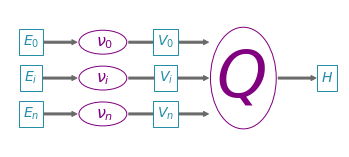
\includegraphics[width=\linewidth]{figures/sections/math/path_of_q.png}
\end{figure}
%%% objects: Data, V, H
%%% functions: \nu, q

We build on top of the existing Matplotlib architecture \cite{hunterMatplotlib2DGraphics2007} so that we can initially focus on the data to graphic transformations and rely on Matplotlib for the other graphical elements of the visualization and the rendering. For a primitive graph such as a bar, scatter, line, our path is: 
\begin{minted}{python}

E = Section()
V = {'parameter': ('field': transformer)}

fig, ax = plt.subplots()
artist = Q(E, V)
ax.add_artist(artist)
\end{minted}



\subsection{Data: $\mathcal{E}$}
We propose a semantic markup of the fiber and connectivity that we will later use to check the constraints of the $\nu$ and $Q$. 
\begin{minted}{python}
class FiberBundle:
    def __init__(self, K, F):
            """
            K: {'tables':[]}
            F: {'field name': (type, monoid action)}
            """

    def is_section(self, section):
        """checks if a section is from a given fiber bundle:
        are values in F, are keys in K"""
        pass
\end{minted}
We add a monoid field to the schema like structure of the fiber since the monoid actions are the constraints on the $\nu$ and $Q$. We implement $K$ using the triangulization scheme described in section~\ref{sec:triangulization}. This means we expect data to be provided as tables where the name encodes the connectivity:

\begin{description}
    \item[vertex] - disconnected points
    \item[edge] - 1D continuity along the edge
    \item[face] - 2D continuity along the face
\end{description}
Nested continuity is encoded in the fiber. For example, one way to encode a movie is a 1D timeseries of \mathrm{Frame} objects, where each \mathrm{Frame} is a $n\x m$ continuous array. 

\subsubsection{Sections}
As described in section~\ref{sec:section_data}, the data values are encode as the section of the fiber bundle. We implement this as as a wrapper class around a data container object of the form:
\begin{minted}{python}
class Section:
    FB = FiberBundle(K, F)

    def __init__(self, *args):
        pass
    def view(self, simplex="vertex"):
        #convert data into atomic column order 
        return {fieldname: data}
\end{minted}

The view function is the closest analog to $\tau$, as it returns a a data container type object. We specify field based top level indexing so that we can pair the fields with transformer $\nu$ objects. 

\subsection{Encoding: $\mathcal{V}$}
We implement $\nu$ as encoder objects with an optional `__init__` method that can be used to specify the range of target visual variables. 

\begin{minted}{python}
class Encoder:
    def __init__(self, args):
        pass
    def validate(self, monoid):
        #check if transform supports monoid action
        pass
    def convert(self, value):
        # convert value to libraries internal normalized form
        pass
\end{minted}

The \mathrm{validate} method specifies the monoids for which this a valid $\nu$ and checks against the specification in the fiber. The \mathrm{convert} method converts a value from data space to an internalized normal form as described in table~\ref{tab:mpl_visual_variable_fiber}.  

\subsection{Graphic: $\mathcal{H}$}
We inherent from the current Matplotlib artists for our $Q$, which is responsible for constructing a curried fully specified internal representation of the graphic.
\begin{minted}{python}
class Q(BaseClass):
    required = {}
    optional = {}
    def __init__(self, data, *args, kwargs):
        # check that required and optional visual parameters are passed in
        # check that the transforms can be applied to the data 
        pass
    def draw(self, render, *args, **kwargs):
        # get frozen atomic section of the data 
        # apply  transforms data
        # set internal attributes of the graphic q generates
        #hands off to backends to draw on screen
        super().draw(renderer, *args, **kwargs)
\end{minted}
While equation~\ref{eq:artist} specifies that the values of $\mu$ can be generated before they are input to $Q$, we curry the opertaions of obtaining the data and performing the transforms to the draw method because that allows us to more easily propogate updates to the data to the screen. 


\subsection{Case Study: Iris(Penguins)}



\end{document}